\section{Initial design}%
\label{sec:org68fdd80}

Following an analysis of the product’s family tree (remote controlled cars), the state of the art and the QFD matrix in fig.~\ref{fig:QFD}, an initial design of the product itself can be produced (fig.~\ref{fig:initial-design}).
The selected approach was top-down, in the sense that the requirements and specifications were addressed and that resulted in a general diagram of the product concept. Some macro-level decisions were made in this stage to narrow the problem’s solutions pool, as follows:

\begin{itemize}
\item  The car itself should be battery-powered, as it is a free-moving object that is intended to work in environments where trailing cables could interfere with its regular movement.

\item The device used to control the car should ideally be one already owned by the user, with an integrated screen (e.g. smartphone), as it would make it more affordable and have a more straightforward interface.

\item The protocol for communication between the controlling device and the Rover should be chosen from within the pool of those readily available to smartphones (e.g. Wi-Fi, GPRS) to keep the price of the overall product down and make it as practical as possible.

\item  The control and communication unit for the car should be divided into two modules: one which can interface directly with the camera module and manage data transmission and reception at the applicational level of the TCP/IP protocol stack, with enough throughput for the specified video resolution and framerate. And another one which can measure and process sensor inputs and control the actuators in real-time.

\end{itemize}

\begin{figure}[!ht]
\centering
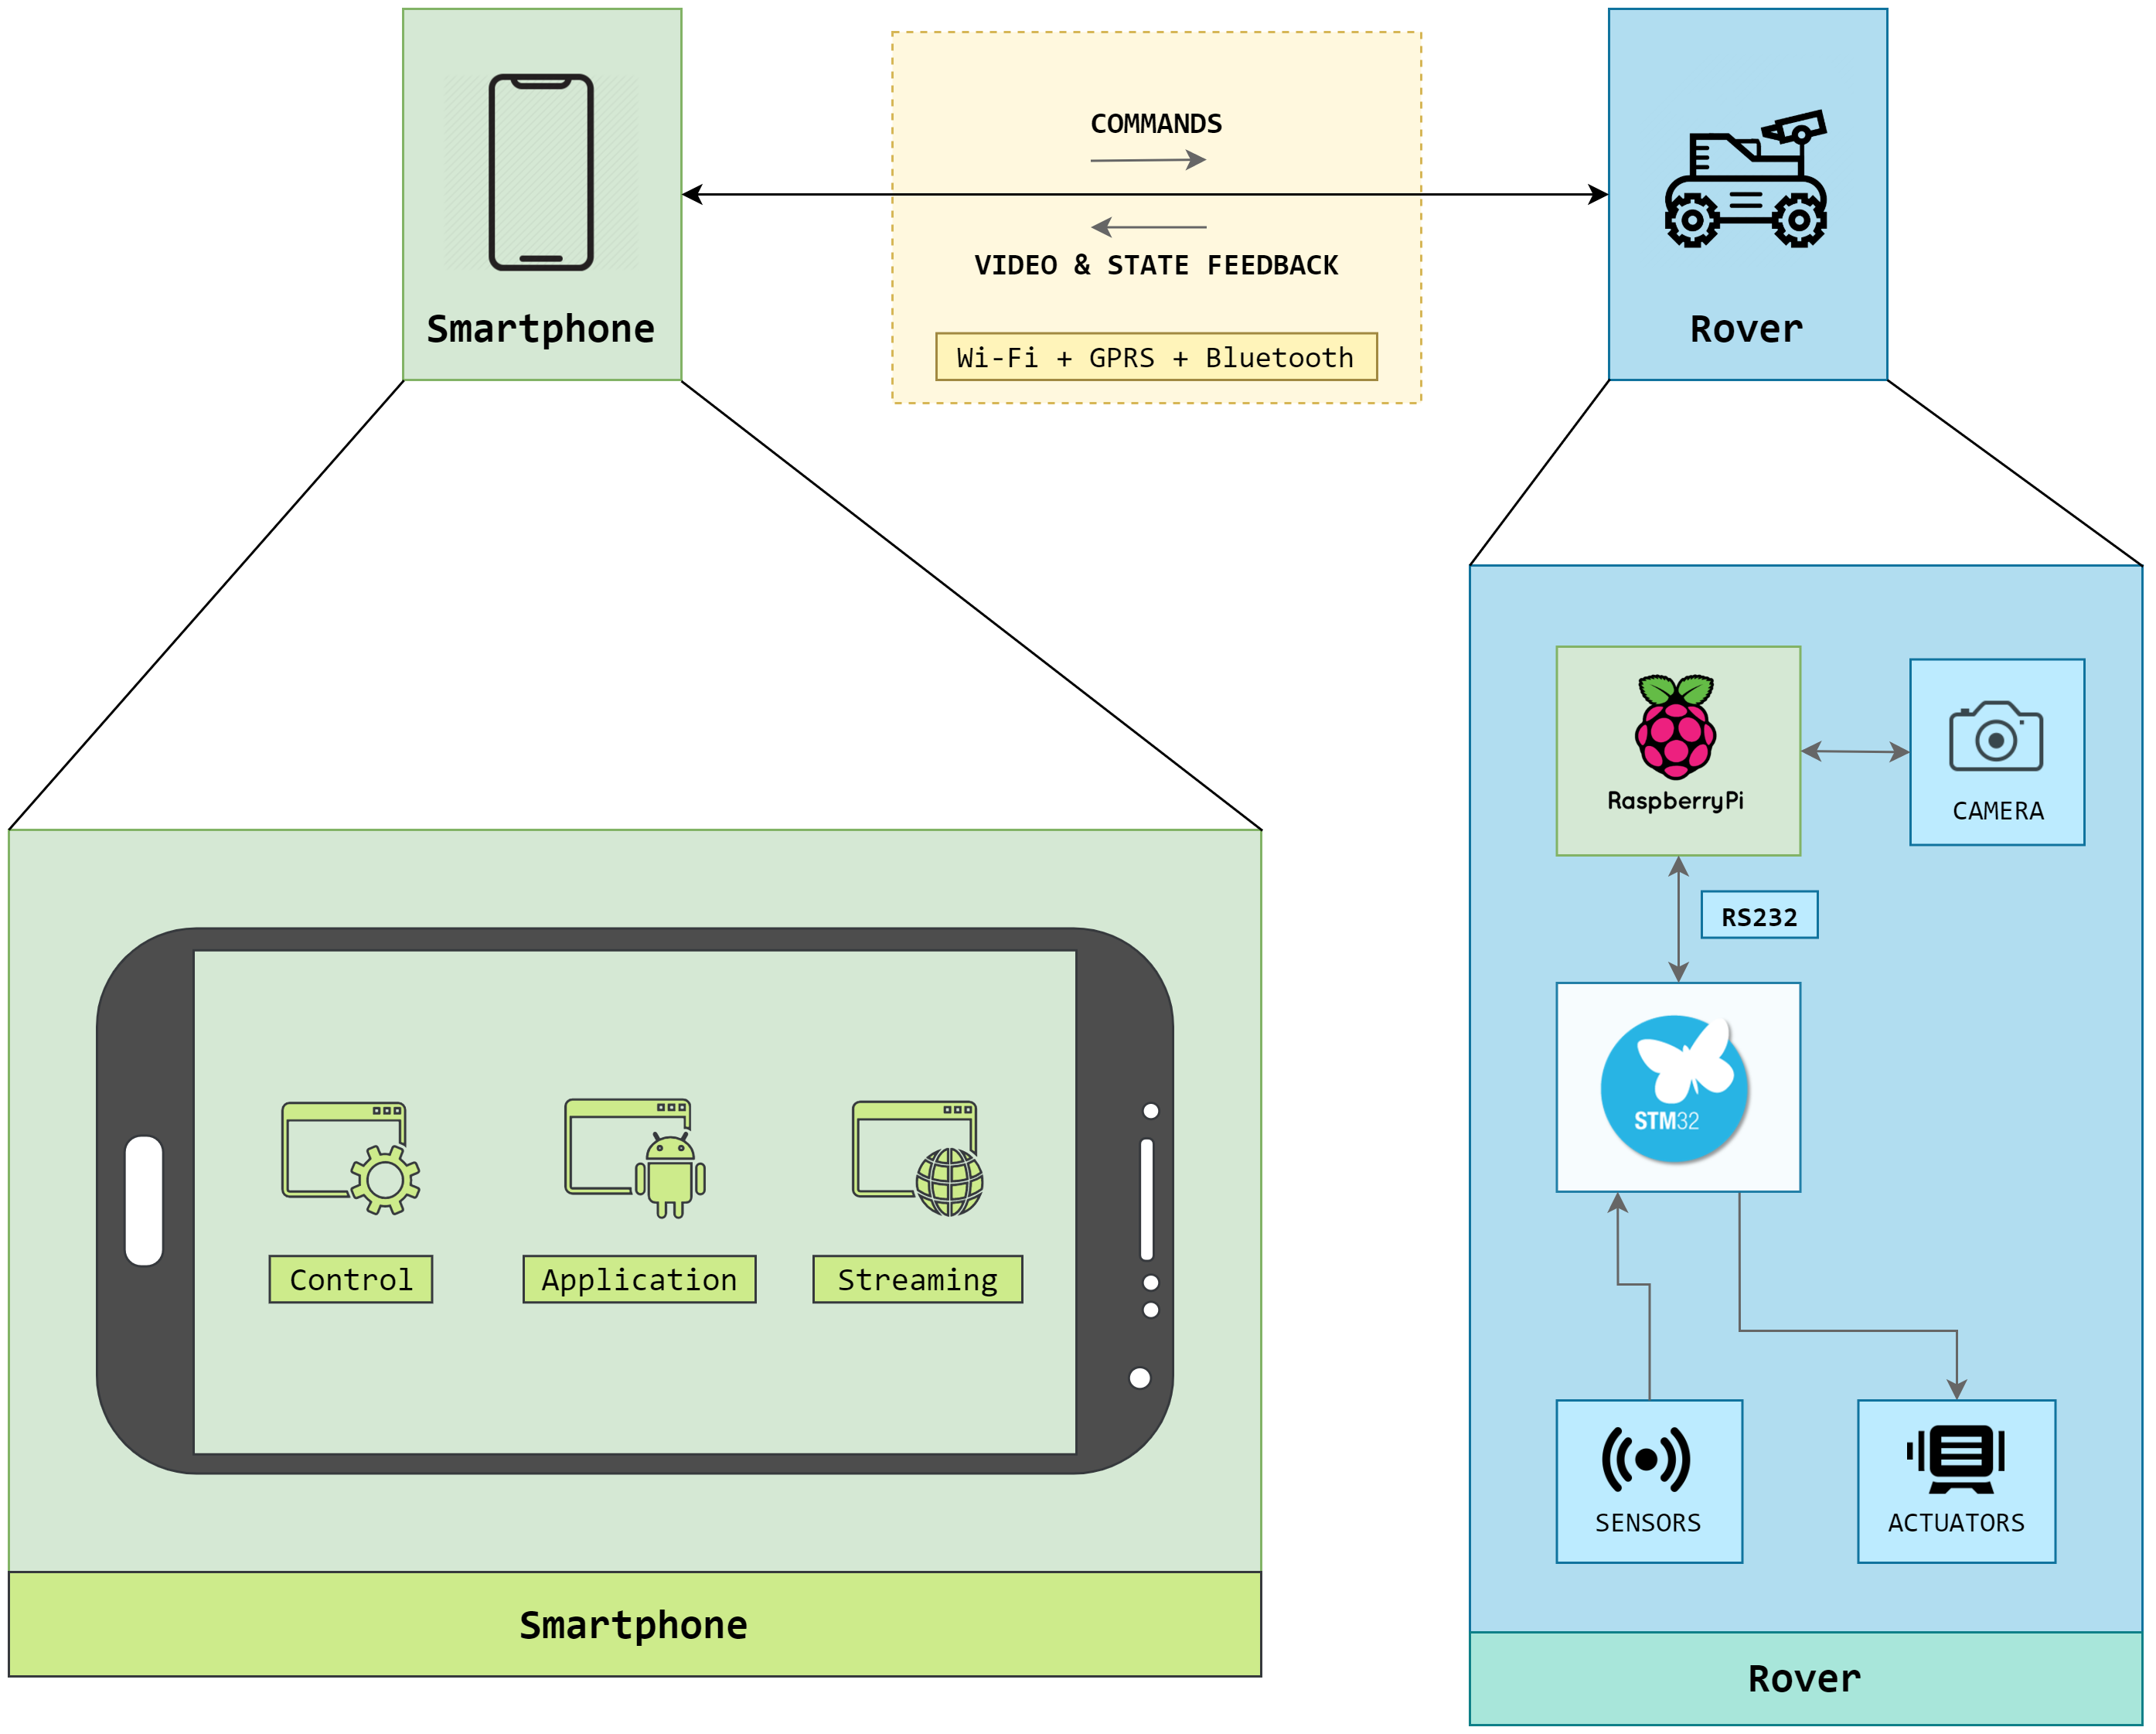
\includegraphics[width=1.0\textwidth]{./sec/img/initial_design_diagram.png}
\caption{\label{fig:initial-design}Initial design: Block diagram view}
\end{figure}

Thus, summarising, the initial design yields the system illustrated in
fig.~\ref{fig:initial-design}, comprised of:

\begin{itemize}
\item \textbf{ Raspberry Pi}: Interfaces with the camera directly, transmitting the information it receives to the smartphone. Receives user commands and sends sensorial information back to it;

\item \textbf{STM32}: Sends sensorial information to the Raspberry Pi module and receives commands from it. Controls the actuators according to the given instructions and sensor readings;

\item \textbf{Actuators}: DC Motors that control the car´s movement and headlights for nocturnal or low light conditions;

\item \textbf{Sensors}: Odometric sensors that supin this senseport the detection of obstacles and luminosity sensors;

\item \textbf{Camera}: Device connected to the Raspberry Pi that allows the live stream of the car´s surrounding environment;

\item \textbf{Smartphone}: Grant visual feedback from the camera´s live feed also allowing the user to control the movement of the vehicle intuitively;

\end{itemize}

Due to the extraordinary conditions imposed by the recently enacted confinement measures, the need rose to create a non-physical connection between both modules of the Rover. For that purpose, a network comprised of two computers communicating over a TCP/IP connection served as the intermediary, one being the Raspberry Pi module and another being a computer connected to the STM32 module via RS232 (fig.~\ref{fig:initial-design-2})

\begin{figure}[!ht]
\centering
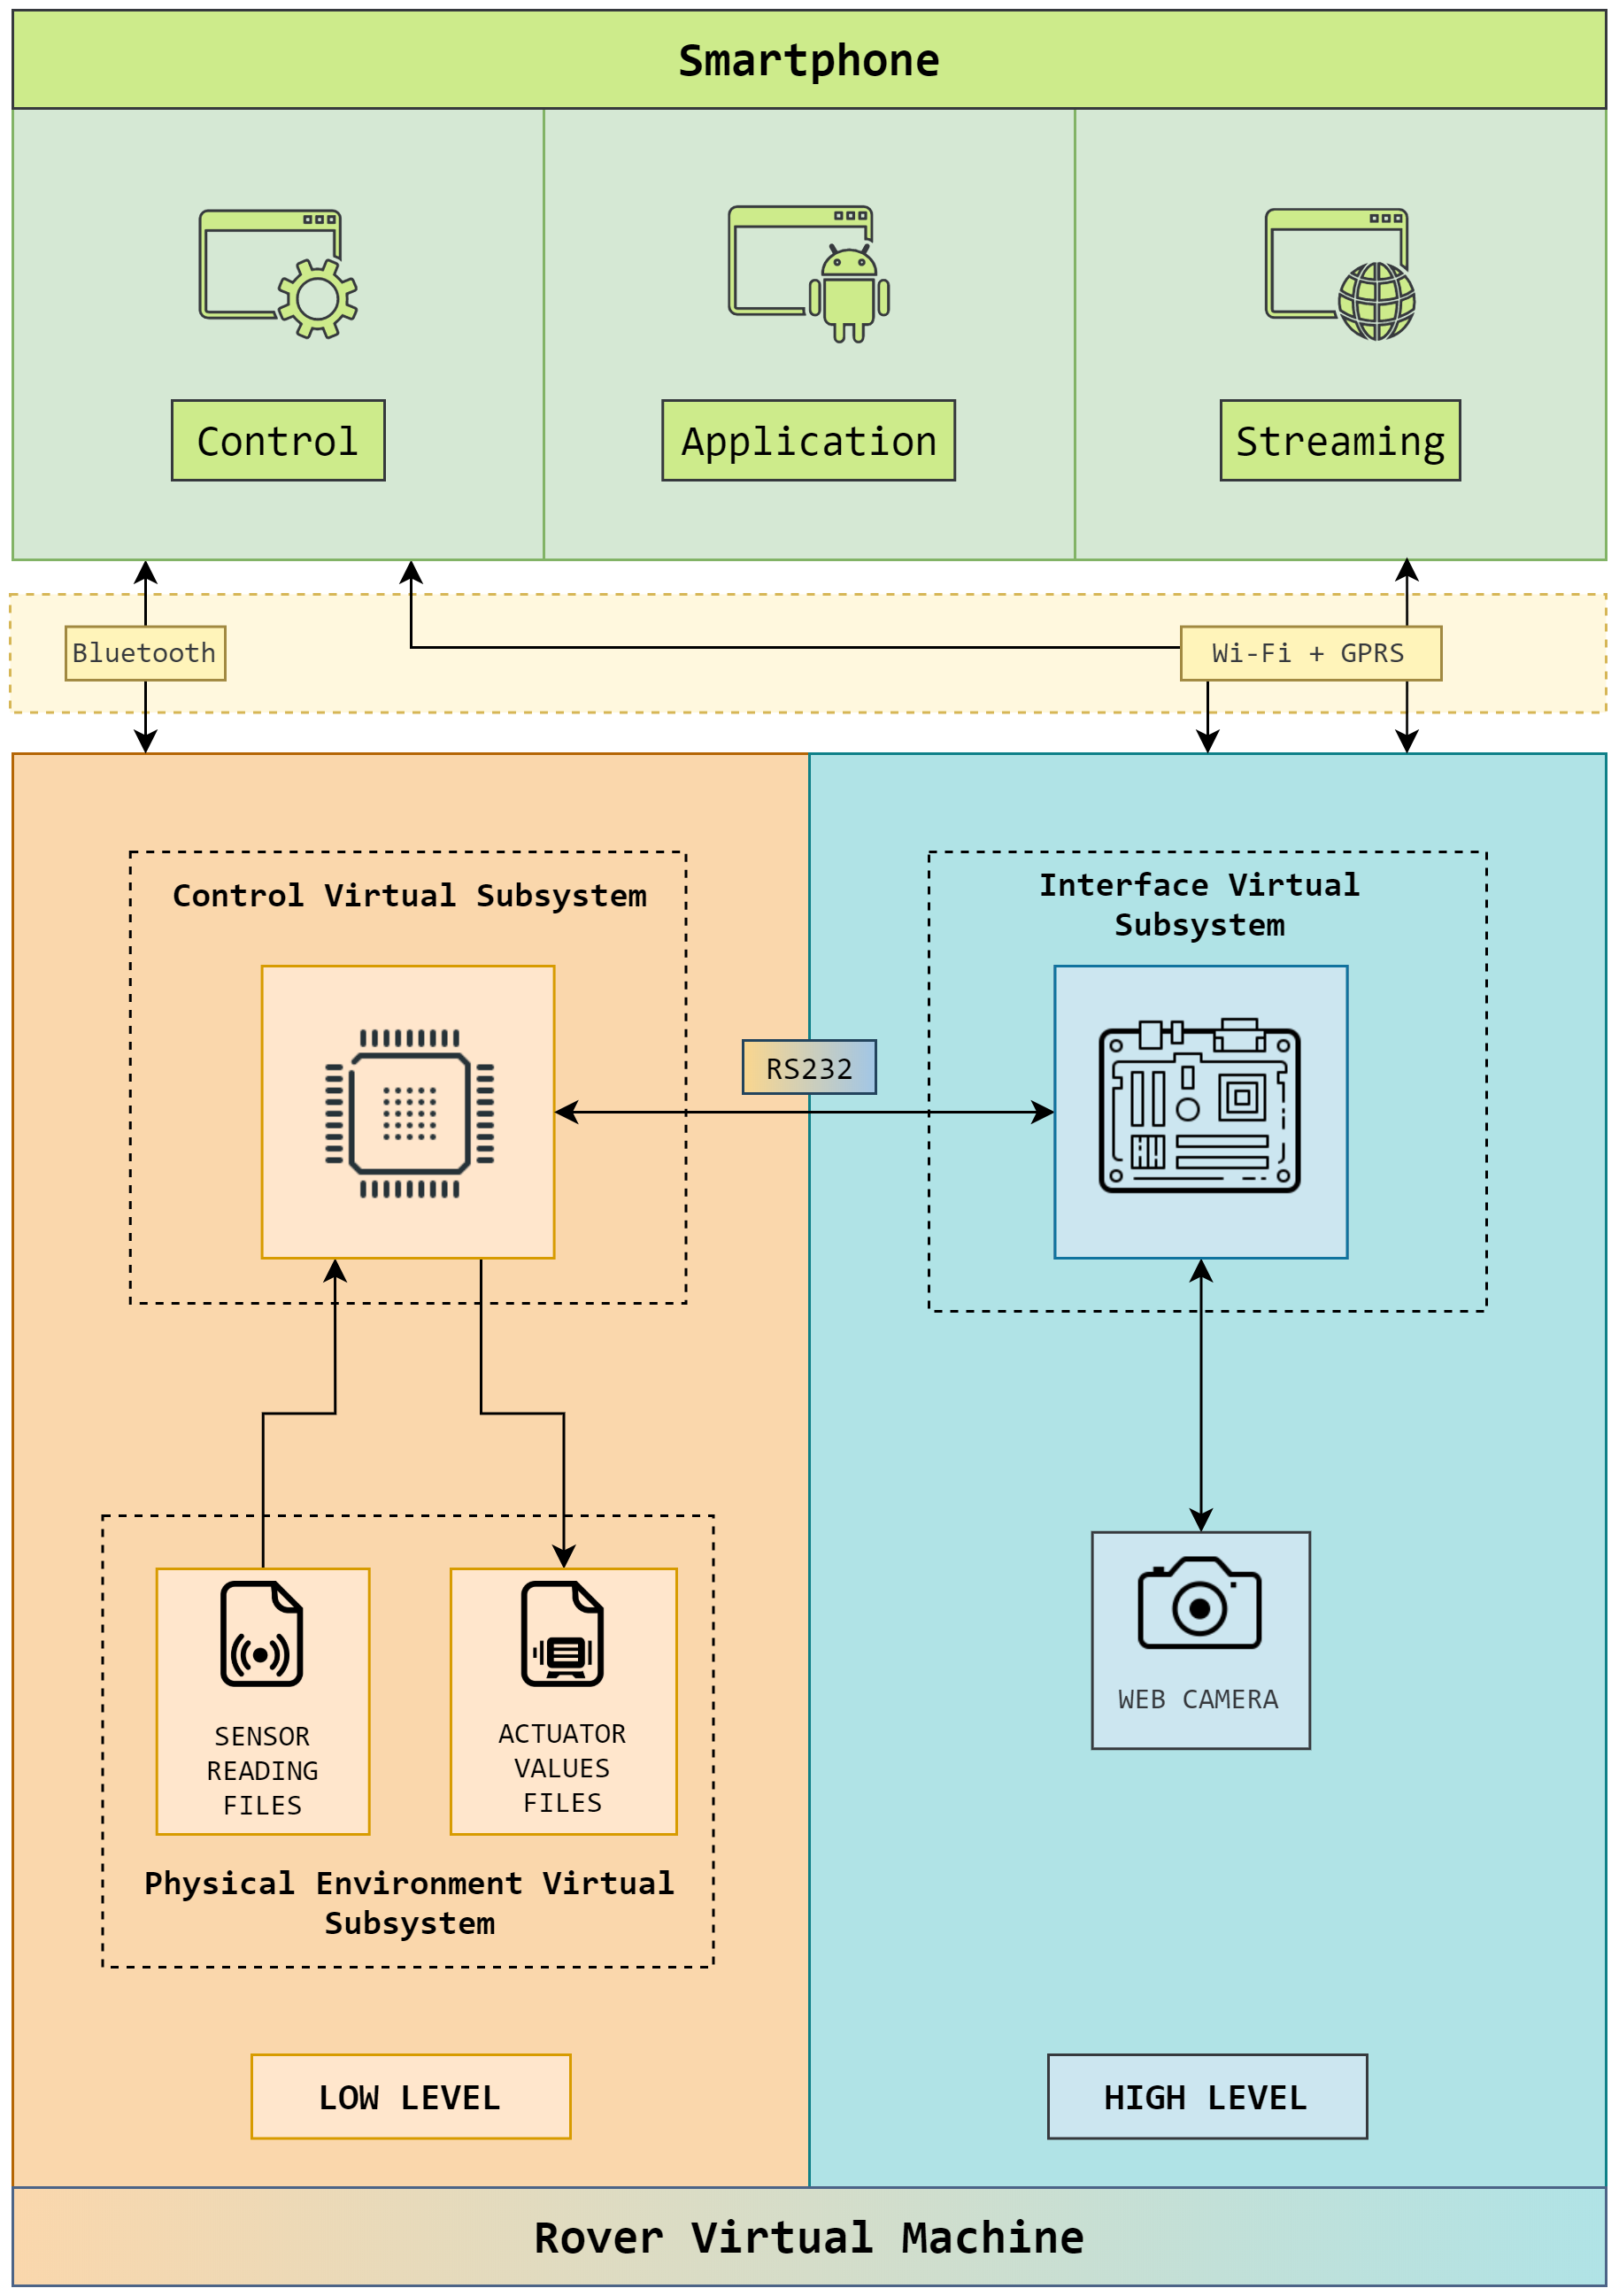
\includegraphics[width=1.0\textwidth]{./sec/img/initial_design_diagram_2.png}
\caption{\label{fig:initial-design-2}Initial design: Block diagram view considering the extraordinary conditions}
\end{figure}

%%% Local Variables:
%%% mode: latex
%%% TeX-master: "../Phase1"
%%% End: